\section{Dataset}\label{sec:dataset}

\subsection{Equation database}\label{sec:db}

We built a database of \NEq{} equations from \NSources{} sources. A source is one PDF file or one
generated equation set. Of the sources, \NPdf{} are PDF files of papers, textbooks, and reports and
contribute \NEqPdf{} equations: \NEarly{} files that we collected early in this work, on continuous
stirred-tank reactors, biodiesel reactions, and process control, and \NOpenAlex{} files that
searches of a scholarly database retrieved for \NFields{} fields, from reaction engineering and heat
transfer to electrochemistry and acoustics (\ref{app:collection}). The other \NRefSets{} sources are
equation sets that Gemini 2.5 Pro \citep{Gemini25} generated field by field to cover textbook
fundamentals; their \NEqRef{} equations have no source document.

A large language model (LLM), Gemini, extracted the equations: Gemini 2.5 Pro for \NExtractPro{} of
the PDF files, and a version of Gemini that no record names for the \NExtractEarliest{} earliest
ones. The model read the PDF and wrote out its numbered equations in \LaTeX{}; for each equation it
returned the variable symbols with their definitions, a context text that explains the physical
meaning of the equation from the surrounding passage, and a domain label (\ref{app:prompts}). The
model kept the symbols as printed, and we normalized none of them, except that a rule added the
Laplace variable $s$ and time $t$ to the variable sets of \NRuleAdded{} equations.

Two properties of the database bear on every later result. First, the database holds \NSymbols{}
distinct variable symbols, and the method matches variables by symbol alone. Of the
\NSymbolsShared{} symbols that appear in two or more equations, \NSymbolsConflict{} carry
definitions that differ between equations. Most differences paraphrase one quantity, but some
symbols name different quantities: $k$ denotes a reaction rate constant, a thermal conductivity,
and a wavenumber in different equations. The method treats each such symbol as one variable.
Second, the domain labels are free text written by the language model, not entries of a fixed
taxonomy: the equations carry \NLabels{} distinct labels, \ShareLabelsOnce\% of which occur once,
so two labels rarely agree exactly.

\subsection{Cases}\label{sec:cases}

Each case pairs a query with a ground-truth equation set for the requested model. We formed
the ground truths in three ways, which gives three families of cases (Table~\ref{tab:families} and
Fig.~\ref{fig:dataset}); the evaluation uses \NCases{} cases. Every case takes its input and output
variables from the symbols of its ground-truth equations, so a query and its answer share one
notation.

\begin{table}[tbp]
\centering
\caption{The three families of evaluation cases. ``Equations'' gives the mean and, in parentheses,
the maximum number of ground-truth equations per case, and ``Sources'' the mean number of sources
that a ground truth draws on.}
\label{tab:families}
\footnotesize
\setlength{\tabcolsep}{4pt}
\begin{tabular}{lp{0.40\linewidth}rcc}
\toprule
Family & How the ground truth was formed & Cases & Equations & Sources \\
\midrule
Single-source & A language model picked a set it judged sufficient and minimal & \NSingle & \MeanKSingle{} (\MaxKSingle) & \MeanSrcSingle \\
Cross-source  & We combined two or three equations from different sources & \NCross & \MeanKCross{} (\MaxKCross) & \MeanSrcCross \\
Synthesized   & A program grew a set from a differential equation to a prescribed size & \NSynth & \MeanKSynth{} (\MaxKSynth) & \MeanSrcSynth \\
\bottomrule
\end{tabular}
\end{table}

\begin{figure}[tbp]\centering
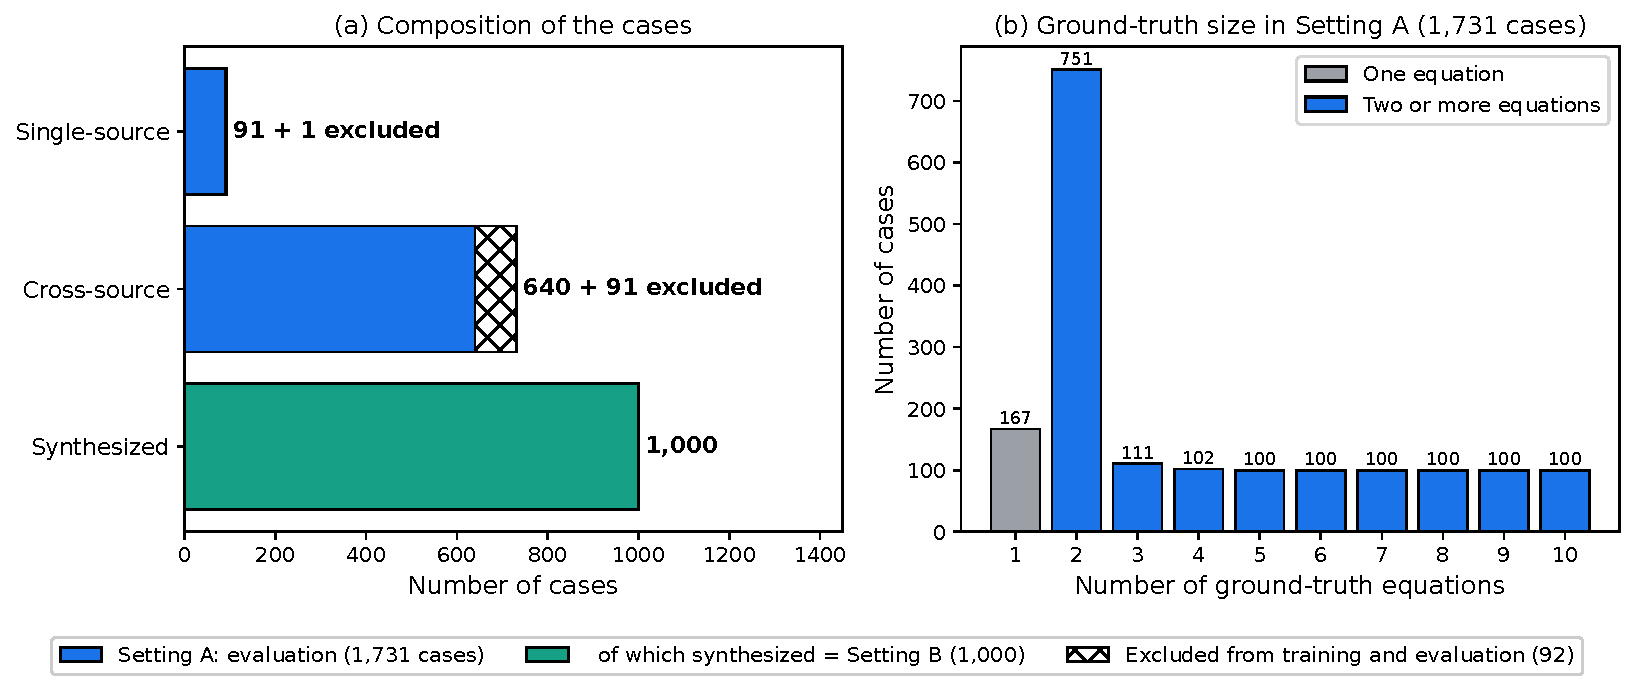
\includegraphics[width=0.98\linewidth]{figures/fig_dataset.pdf}
\caption{The evaluation cases. (a) Composition: Setting~A uses the single-source, cross-source, and
synthesized cases, and Setting~B the synthesized cases alone; hatched bars mark the cases excluded
from training and evaluation. (b) Number of ground-truth equations per case in Setting~A.}
\label{fig:dataset}
\end{figure}

A language model formed the ground truths of the single-source family (\NSingle{} cases). We gave
Gemini 2.5 Pro a catalog of the database as it then stood, which listed for each equation only
its domain label, its variable symbols, and its identifier, which names its source, and asked for
physically meaningful cases: a description, input and output
variables, and a ground-truth set that the inputs determine and that is sufficient and minimal
(\ref{app:prompts}). We kept the cases whose ground-truth equations all exist in the database, whose
input and output variables all appear in them, and whose ground truth has as many unknowns as
equations once the inputs are given. Each ground truth draws on one source. It is the set that the
model judged minimal, not a model that a source presents; \NSingleOneEq{} of the \NSingle{} ground
truths hold a single equation, and \NSingleRefOnly{} draw only on the generated equation sets.

The cross-source family (\NCross{} cases) combines two or three equations from different sources. A
program built \NCrossProgram{} of these cases. It grouped the domain labels into ten categories,
such as reactor, heat transfer, and control, by hand-written word lists; took pairs of categories
that chemical engineering often combines; collected pairs of equations that come from different
sources and share at least two variable symbols; and formed cases whose outputs are one variable
unique to each equation and whose inputs are all other variables. It wrote each description from an
English template. The other cases are \NCrossPicked{} combinations that a coding-assistant language
model (Claude) wrote as physically meaningful and \NCrossReselected{} variants of them with
reselected input and output variables. Claude Opus 4.8 \citep{ClaudeOpus48} rewrote the descriptions
of these variants, and of two of the original combinations, to match their output variables.

A program formed the ground truths of the synthesized family (\NSynth{} cases,
\secref{sec:synth}).

All ground truths meet requirements~1--3 of \secref{sec:formulation}. Because these
requirements only count variables and equations, we also checked that each unknown can be assigned
to an equation of its own. This check, too, only counts: whether the equations then determine the
outputs was judged on a sample alone (\secref{sec:limitations}). We excluded \NExcluded{} generated cases from both training and
evaluation: \NExcludedCross{} cross-source cases in which one ground-truth equation contains input
variables only, so that some unknowns stay undetermined once the inputs are given, and one
single-source case whose ground truth draws on two sources. Requirement~3 holds trivially in
\NReqThreeTrivial{} of the \NCases{} cases, which contain no variable other than the inputs and
outputs, and requirement~4 cannot be checked, because the database does not mark which variables are
constants. Over all cases, \ShareKTwoPlus\% have two or more ground-truth equations, and the mean is
\MeanKAll.

\subsection{Synthesized cases}\label{sec:synth}

The ground truths of the first two families hold at most \MaxKSingle{} equations, so a program
generated larger ones that mix differential and algebraic equations. It fixes a target size $X$ and
works in two phases. First, it picks a differential equation of the database at
random and takes one of its differentiated variables as an output. It then repeatedly adds an
equation that contains a variable, other than that output, of the equations collected so far,
choosing at random among the equations of the first equation's source when any qualifies and among
those of other sources otherwise, until the set holds $X$ equations. Second, it goes through the
added equations, chooses at random one variable of each that is not yet an output, and adds it to
the outputs; every variable left over becomes an input. The resulting sets have as many unknowns as
equations once the inputs are given, and each equation contributes an output of its own, so every
unknown can be matched to its own equation. We generated 100 cases for each $X$ from 1 to 10;
\NSynthOneSource{} of the \NSynth{} cases draw on a single source. A language model, Claude Sonnet
4.5 \citep{ClaudeSonnet45}, wrote only the description of each case; the equation set, the inputs,
and the outputs all follow from the program (\ref{app:example} shows one case).

\subsection{Stratified split by source}\label{sec:split}

We split the cases into training, validation, and test cases by source. We assign each case to the
source that contributes most of its ground-truth equations, and each source goes wholly, with the
cases assigned to it, to one part: 20\% of the sources to testing, 20\% to validation, and 60\% to
training. Two cases assigned to the same source therefore never fall into different parts. A ground
truth that draws on several sources, however, can share equations with the cases of another part.
In Setting~A, \ShareSharedEqA\% of the test cases of the 10 splits share at least one ground-truth
equation with a training case (\ShareSharedEqAMin\% to \ShareSharedEqAMax\% per split): \ShareSharedEqCross\%
of the cross-source, \ShareSharedEqSynth\% of the synthesized, and \ShareSharedEqSingle\% of the
single-source test cases. In Setting~B, \ShareSharedEqB\% do. The reranker reads ten features of a
candidate, not its identity, so it cannot memorize an equation; the test cases are nevertheless not
all new to it at the level of equations. \ref{app:overlap} therefore scores the methods separately
on the test cases that share a ground-truth equation with a training case and on those that share
none. Because sources hold different numbers of cases, the numbers of cases
vary from split to split: \NTestAMin{} to \NTestAMax{} test cases and \NValAMin{} to \NValAMax{}
validation cases in Setting~A.

A random assignment of sources can put the cases with many equations on one side, so we stratify
it. For one split, we draw \NSplitCandidates{} random assignments and take four quantities per
case: the numbers of ground-truth equations, of input variables, of output variables, and of
sources spanned. For each quantity we compute the $L_1$ distance between its training and test
frequency distributions, and we select the assignment with the smallest sum of the four distances
(\ref{app:split} shows one split).
Every experiment repeats this procedure over the same 10 random seeds and reports the mean and the
standard deviation across them; the seed also fixes the initialization of the model and the choice
of incorrect candidates. The validation cases choose the hyperparameters of the methods
(\secref{sec:compared}).
